\chapter{Experiments}



\section{Remaining Plots}
	\label{app:remainingPlots}

	In this section we put all plots referenced in~\autoref{sec:results} that where not directly in that section as they do not add much new information.

	\subsection{Gym Cartpole}
		\subsubsection{Exemplary Evaluation: One-Dimensional Latent}
			\begin{figure}
				\centering
				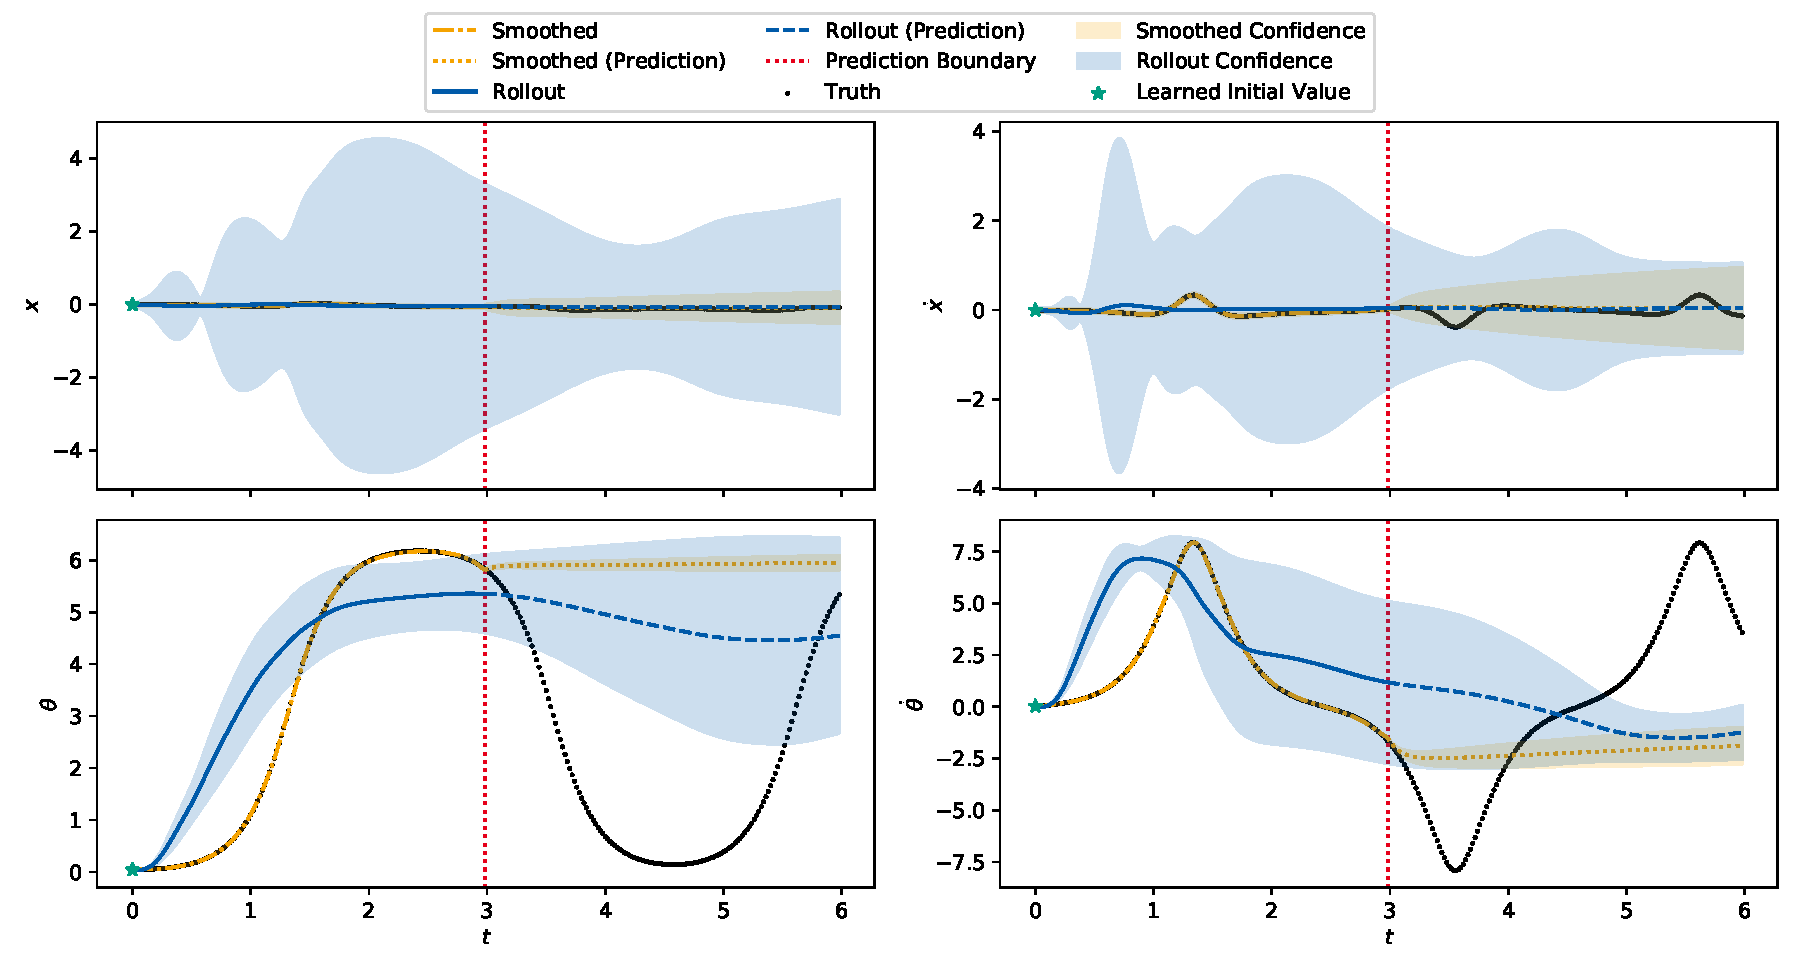
\includegraphics[width=\linewidth]{figures/results/cartpole-gym/run-latent-dim-02/rollout-observations-N0.pdf}
				\caption{This plot shows the same data as in~\autoref{fig:cartpoleRolloutL01}, but with the confidence shown. As the confidence is quite low, this plot is hard to interpret which is the reason why we removed the confidence plot in the first place.}
				\label{fig:cartpoleRolloutL01Appendix}
			\end{figure}

			\begin{figure}
				\centering
				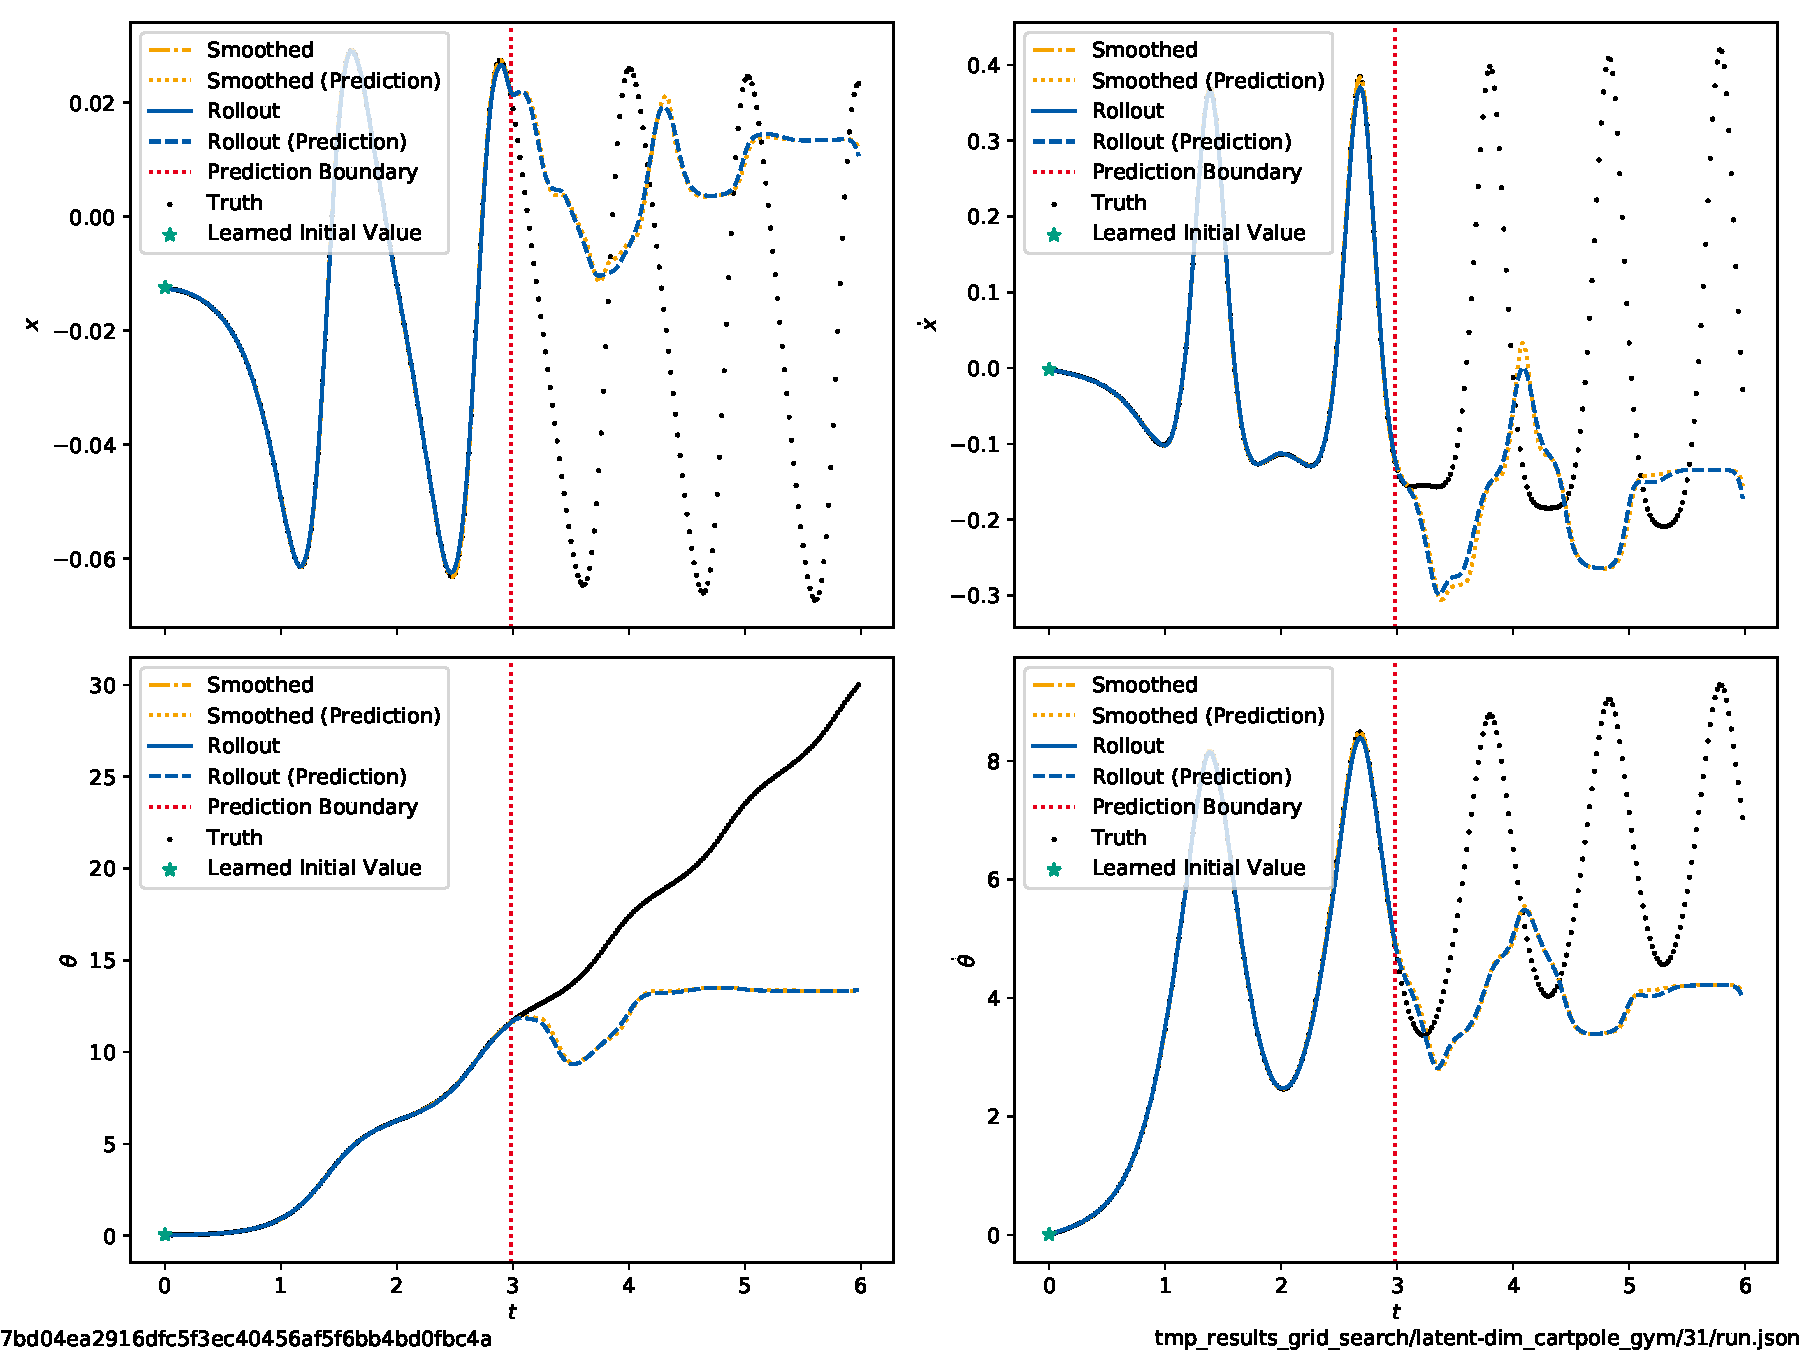
\includegraphics[width=\linewidth]{figures/results/cartpole-gym/run-latent-dim-31/without-confidence/rollout-observations-N0.pdf}
				\caption{This plot shows the same data as in~\autoref{fig:cartpoleRolloutL01}, but without the confidence shown.}
				\label{fig:cartpoleRolloutL10Appendix}
			\end{figure}

			\begin{figure}
				\centering
				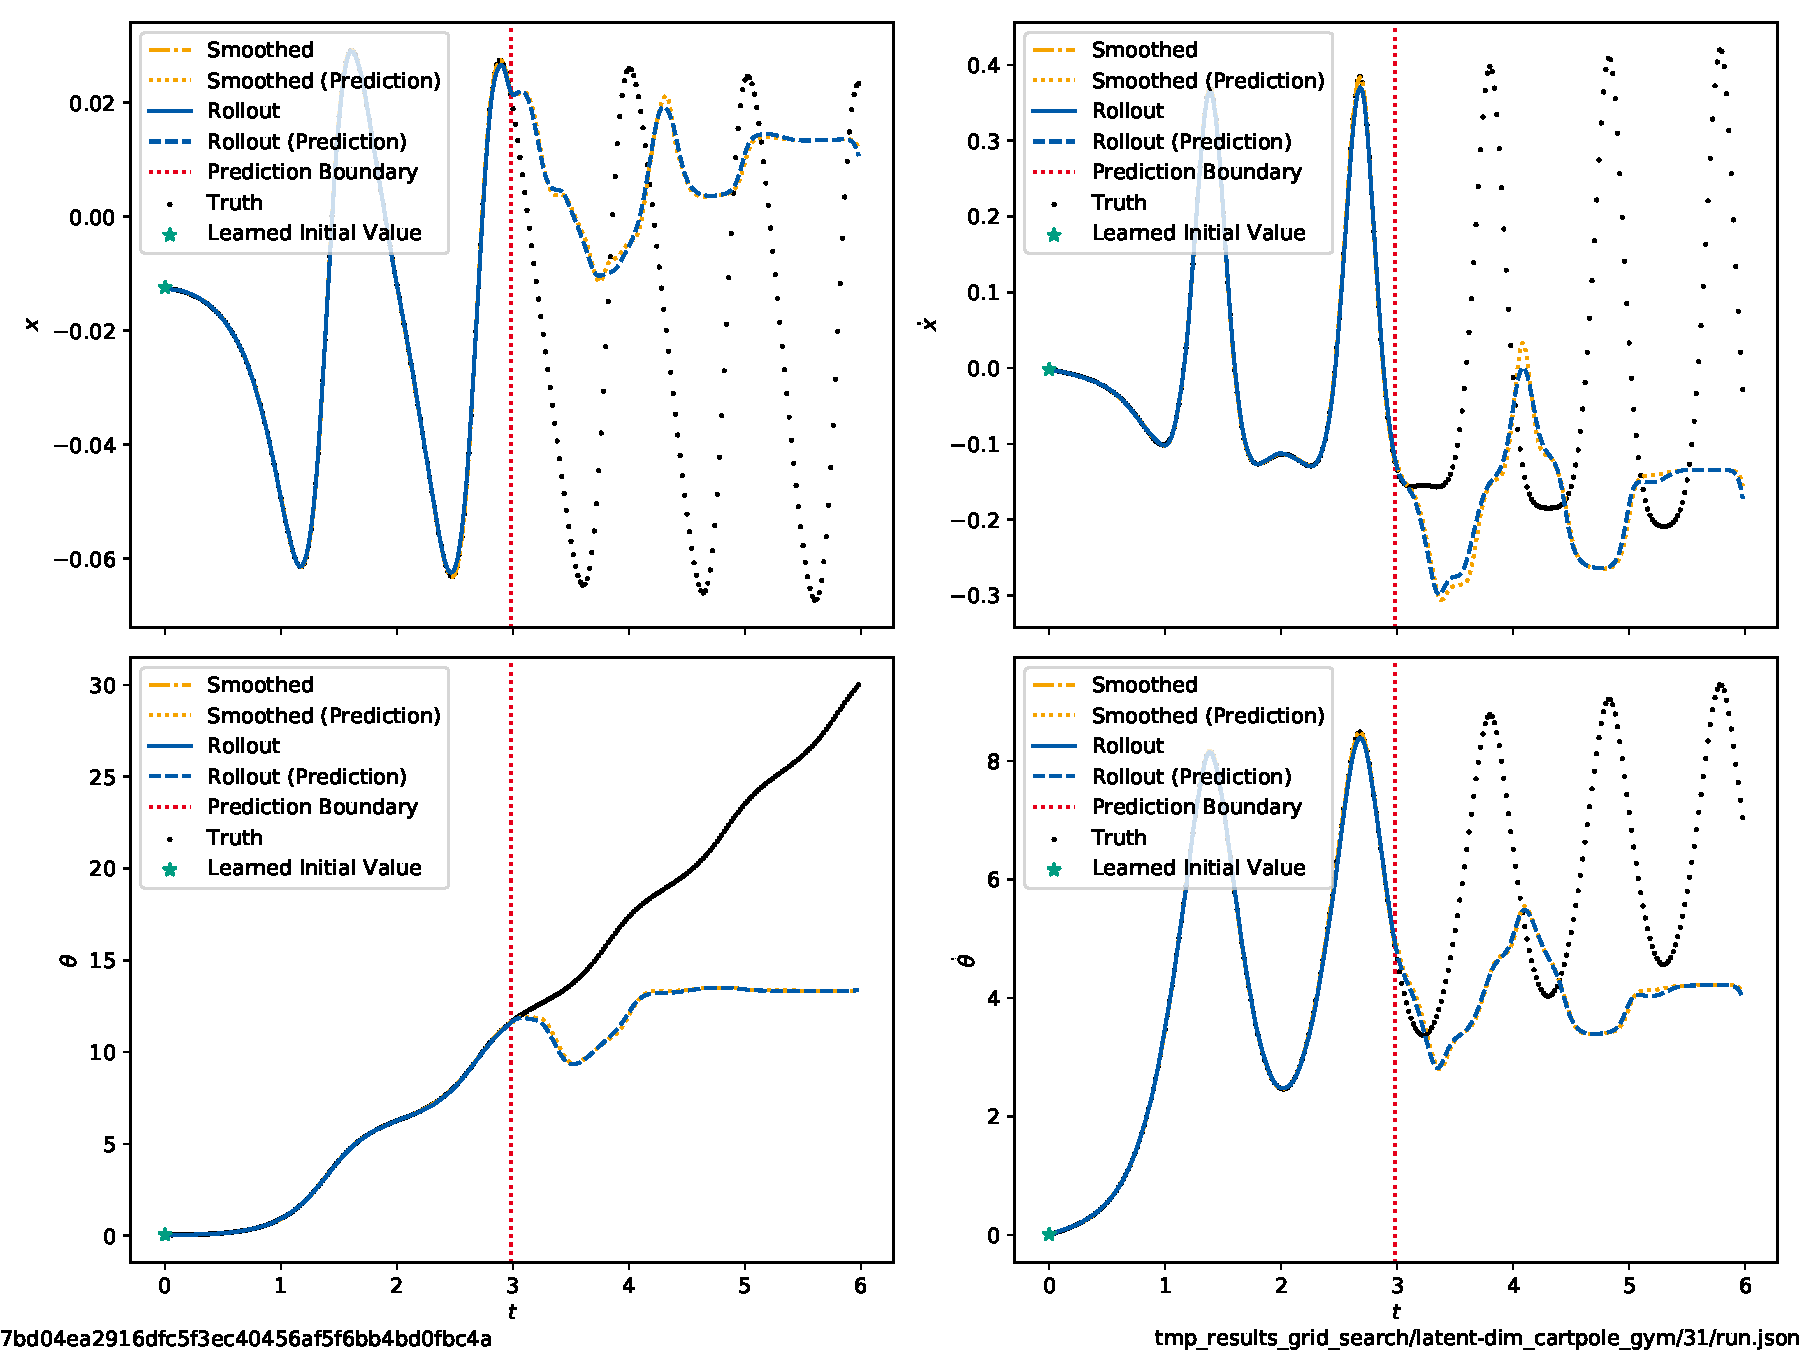
\includegraphics[width=\linewidth]{figures/results/cartpole-gym/run-latent-dim-31/without-confidence/rollout-observations-N0.pdf}
				\caption{This plot shows the same data as in~\autoref{fig:cartpoleRolloutL01}, but without the confidence shown.}
				\label{fig:cartpoleRolloutL31Appendix}
			\end{figure}
		% end
	% end
% end
